\documentclass[a4paper,10pt]{article}
\usepackage[spanish]{babel}
\usepackage[utf8]{inputenc}

\usepackage{color}
\usepackage{amsmath}
\usepackage{graphicx}

\newcommand{\abs}[1]{\lvert#1\rvert}
\newcommand{\norm}[1]{\lVert#1\rVert}
\newcommand{\vect}[1]{\boldsymbol{\vec{#1}}}
\newcommand{\versor}[1]{\boldsymbol{\hat{#1}}}
\newcommand{\attention}[1]{ {\color{red}#1} }
\newcommand{\revisar}[1]{\textcolor{yellow}{#1}}

\title{Una implementación del algoritmo Exposure Fusion bajo el paradigma SIMD}
\author{Kevin Allekotte, Thomas Fischer}
\date{\today}

\begin{document}

    \maketitle

    \begin{abstract}
        Una cámara captura la intensidad de la luminosidad en cada punto de una imagen. El rango de estas intensidades varía según la \emph{exposición} de la cámara (que se controla con la apertura, tiempo de exposición y sensibilidad), pero el tamaño del rango de luminosidades -\emph{rango dinámico}- es acotado. Es decir, se saturan las intensidades para valores fuera de ese rango, perdiendo detalle en esas zonas (partes quemadas -blancas- y oscuras -negras-).
        
        Es posible capturar el rango dinámico completo de una imagen con múltiples fotos con distintas exposiciones y fusionandolas. El objetivo de este trabajo es fusionarlas de manera de producir otra imagen de rango dinámico acotado de la mejor forma posible, ya que los medios para reproducir fotos también son de rango acotado (monitores, impresión).
        
        Se presenta una implementación del algoritmo de Exposure Fusion \cite{DBLP:conf/pg/MertensKR07} en assembler x64 usando SIMD Extensions.

    \end{abstract}

    \section{Introducción}

        El rango dinámico del ojo humano es dificil de calcular, pero bajo condiciones parecidas a las de un sistema de fotografía, está estimado entre 10 a 14 \emph{f-stops}. Vemos la gran diferencia que hay entre un sensor digital y el ojo humano, por lo que reproducir adecuadamente lo que ve un ojo es imposible bajo condiciones de mucho rango dinámico, considerando que un día soleado con reflectividad dispareja tiene un rango de 12+ \emph{f-stops}.

        Las imágenes HDR (High Dynamic Range) son imágenes que tienen un rango dinámico mucho más grande, y por lo tanto resultan más representativas y mas detalladas que las imágenes comunes. HDRI (HDR Imaging) son métodos utilizados para crear imágenes HDR combinando la información de varias imágenes de la misma escena con menor rango dinámico bajo distintas exposiciones.

        Sin embargo, las imágenes HDR no son apropiadas para mostrar en monitores o imprimir, ya que el rango dinámico de estos medios también es acotado y son aptos para ver sólo imágenes con bajo rango dinámico. Una opción, entonces, es volver a \textbf{comprimir una imagen HDR a un rango dinámico acotado, mostrando la mayor cantidad de detalle en cada zona y manteniendo la estética y realismo de la misma}. Hay distintos algoritmos que logran esto con distintos resultados, se llaman algoritmos de \emph{Tone Mapping}.

        Exposure Fusion \cite{DBLP:conf/pg/MertensKR07} es una técnica desarrollada para fusionar varias imágenes de bajo rango dinámico tomadas a distintas exposiciones  con un resultado similar a los operadores de tone mapping de HDR. Esta técnica evita pasos como la creación de la imagen HDR, la calibración de la curva de respuesta de la cámara y la selección de operadores de tone mapping, pasos que son costosos computacionalmente e implican una calibración ''a ojo'' de los parámetros.
        
        Exposure fusion analiza ciertas propiedades de las imágenes que son relevantes para la calidad de la foto, y por cada pixel de la imagen se queda con la ''mejor'' información que puede recuperar a partir de todas las imágenes originales. Estas propiedades son el contraste, la saturación y la calidad de exposición de un pixel. El resultado final es computado automáticamente. A diferencia de otros algoritmos de tone-mapping, no requiere la creación de la imagen HDR sino que directamente combina las distintas exposiciones. Gracias a esto es más robusto, más rapido, y permite por ejemplo mezclar tomas con y sin flash.

    \section{Algoritmo}

        Cada pixel de la imagen final se obtiene como la suma ponderada de los valores de ese pixel en las imágenes de entrada. El peso que se le asigna a cada muestra es la medida de la calidad de ese pixel en esa imagen. En resumen:

        $$ R_{i,j} = \sum_{k=1}^N{ \hat{W}_{k_{i,j}}*I_{k_{i,j}} } $$

        Donde $N$ es la cantidad de imágenes a fusionar, $I_k$ son esas imágenes, $\hat{W}_{k_{i,j}}$ es el peso del pixels $I_{k_{i,j}}$ y $R_{i,j}$ es la imagen resultante.

        Para calcular los pesos $\hat{W}_{k,i,j}$, primero calculamos la calidad de cada pixel en función de las tres propiedades descriptas anteriormente

        $$ W_{k_{i,j}} = (C_{k_{i,j}})^{w_C} \times (S_{k_{i,j}})^{w_S} \times (E_{k_{i,j}})^{w_E} $$

        donde $w_C$, $w_S$ y $w_E$ son parámetros que regulan cuanta importancia le queremos dar a cada métrica, y luego normalizamos los pesos de las matrices $W_{k_{i,j}}$ para que el resultado sume 1 en cada pixel, y el resultado tenga el mismo depth bit que las imágenes originales.

        $$ \hat{W}_{k_{i,j}} = W_{k_{i,j}} \times [\sum_{k'=1}^N{W_{k'_{i,j}}}]^{-1} $$ 

        Nos falta entonces calcular las matrices de calidad respectivas a cada propiedad.

        \subsection{Contraste}

            Aplicamos un filtro laplaciano a la versión en escala de grises de cada imagen y nos quedamos con el valor absoluto de la respuesta. Esto suele asignar pesos altos a elementos que pertenecen a bordes o texturas en la imagen.

        \subsection{Saturación}

            Una medida importante de la calidad de la imágen es la saturación. Buscamos colores vívidos, que son los que tienen más diferencia entre los colores que lo componen. Se calcula como la desviación estandar del componente rojo, verde y azul. ($\frac{\sqrt{(r-\mu)^2 + (g-\mu)^2 + (b-\mu)^2}}{3}$, $\mu = \frac{b+g+r}{3}$).

        \subsection{Exposición}

            Una pixel bien expuesto es aquel que no tiene una intensidad cercana al mínimo o al máximo (sobresaturada) del rango dinámico. Luego, definimos la calidad de la exposición como la distancia al valor óptimo $0.5$, siguiendo una curva gaussiana $exp(-\frac{(i-0.5)^2}{2\sigma^2})$, donde proponemos $\sigma = 0.2$ como en \cite{DBLP:conf/pg/MertensKR07}. En imágenes de color aplicamos esta función por cada canal y multiplicamos los resultados.

    \section{Implementación}

        La aplicación esta hecha para Linux de 64 bits (fue probado en distintas versiones de Ubuntu). El principal lenguaje de programación usado en la implementación fue C. Las operaciones de procesamiento de las imágenes fueron implementadas en ASM x64 para mejorar la performance, y se utilizó GTK para la interfaz gráfica. Para cargar y guardar imágenes se usa la librería OpenCV.
        
        Se abstrayeron las operaciones sobre matrices en el módulo \texttt{Matrix}, los algoritmos del Exposure Fusion están en \texttt{Expofuse}, y la interfaz gráfica en \texttt{Gui}. Los 3 módulos están implementados en C, y \texttt{Matrix} y \texttt{Expofuse} hacen llamadas a código en assembler en muchas de las funciones.
        
        \subsection{\texttt{Matrix}}
            El tipo Matrix es una \texttt{struct} de este tipo:
            
            \begin{verbatim}
            typedef struct {
              int cols;
              int rows;
              double* data;
            } Matrix;\end{verbatim}

            y implementa las siguientes operaciones:
            
            \texttt{Matrix* NewMatrix(int rows, int cols)}
            
            \texttt{void DeleteMatrix(Matrix* A)}
            
            \texttt{Matrix* CopyMatrix(Matrix* A)}
            
            \texttt{Matrix* Substract(Matrix* A, Matrix* B)}
            
            \texttt{Matrix* AddMatrix(Matrix* A, Matrix* B)}
            
            \texttt{Matrix* AddEqualsMatrix(Matrix* A, Matrix* B)}
            
            \texttt{Matrix* Convolve(Matrix* A, Matrix* kernel, BOUNDARY)}
            
            \texttt{Matrix* Downsample(Matrix* I)}
            
            \texttt{Matrix* Upsample(Matrix* I, int odd\_rows, int odd\_cols)}
            
            \texttt{void ContrastCurve(Matrix* A, double strength)}
        
        \subsection{\texttt{Expofuse}}
            Para representar imágenes y procesarlas usamos una \texttt{struct} de este tipo:
            
            \begin{verbatim}
            typedef struct {
              Matrix* R;
              Matrix* G;
              Matrix* B;
            } ColorImage;\end{verbatim}
            
            con las funciones:
            
            \texttt{ColorImage* NewColorImage()}

            \texttt{void DeleteColorImage(ColorImage* image)}

            \texttt{ColorImage* CopyColorImage(ColorImage* image)}

            \texttt{ColorImage* AddColorImage(ColorImage* A, ColorImage* B)}

            \texttt{ColorImage* AddEqualsColorImage(ColorImage* A, ColorImage* B)}

            \texttt{ColorImage* LoadColorImage(char* filename, int size)}

            \texttt{void SaveColorImage(ColorImage* I, char* filename)}

            \texttt{void TruncateColorImage(ColorImage* I)}

            \texttt{void SContrast(ColorImage* A, double strength)}
            
            \bigskip
            y para implenetar Exposure Fusion se tienen las funciones:
            
            \texttt{Matrix** ConstructWeights(ColorImage** color\_images, int n\_samples, double contrast\_weight, double saturation\_weight, double exposeness\_weight, double sigma)}
            
            \texttt{Matrix* Contrast(Matrix* I)}

            \texttt{Matrix* Saturation(ColorImage* I)}

            \texttt{Matrix* Exposeness(ColorImage* I, double sigma)}

            \texttt{Matrix* Weight(Matrix* contrast, double contrast\_weight, Matrix* saturation, double saturation\_weight, Matrix* exposeness, double exposeness\_weight)}

            \texttt{void NormalizeWeights(Matrix** weights, int n\_samples)}

            \texttt{void WeightColorImage(ColorImage* color\_image, Matrix* weights)}

            \texttt{ColorImage* Fusion(ColorImage** images, Matrix** weights, int n\_samples)}

            \texttt{Matrix** GaussianPyramid(Matrix* I, int levels)}

            \texttt{Matrix** LaplacianPyramid(Matrix* I, int levels)}

            \texttt{ColorImage** ColorLaplacianPyramid(ColorImage* I, int levels)}

            \texttt{ColorImage* ReconstructFromPyramid(ColorImage** pyramid, int n\_levels)}
            
            \bigskip
            Para las partes en Assembler, implementamos la convención de llamadas a funciones de C en x64 y creamos las funciones que nos interesaban. Usamos las extensiones SSE para la mejor performance, y implementamos casos específicos para optimizar las operaciones más demandantes.

    \section{Resultados}

        Tal como los resultados de Mertens, Kautz y Van Reeth, obtuvimos imágenes con mucho nivel de detalle en condiciones de mucho contraste y alto rango de luminosidad, que son estéticas y muy realistas. A continuación mostramos algunos resultados con las imágenes de entrada y la composición final.
        
        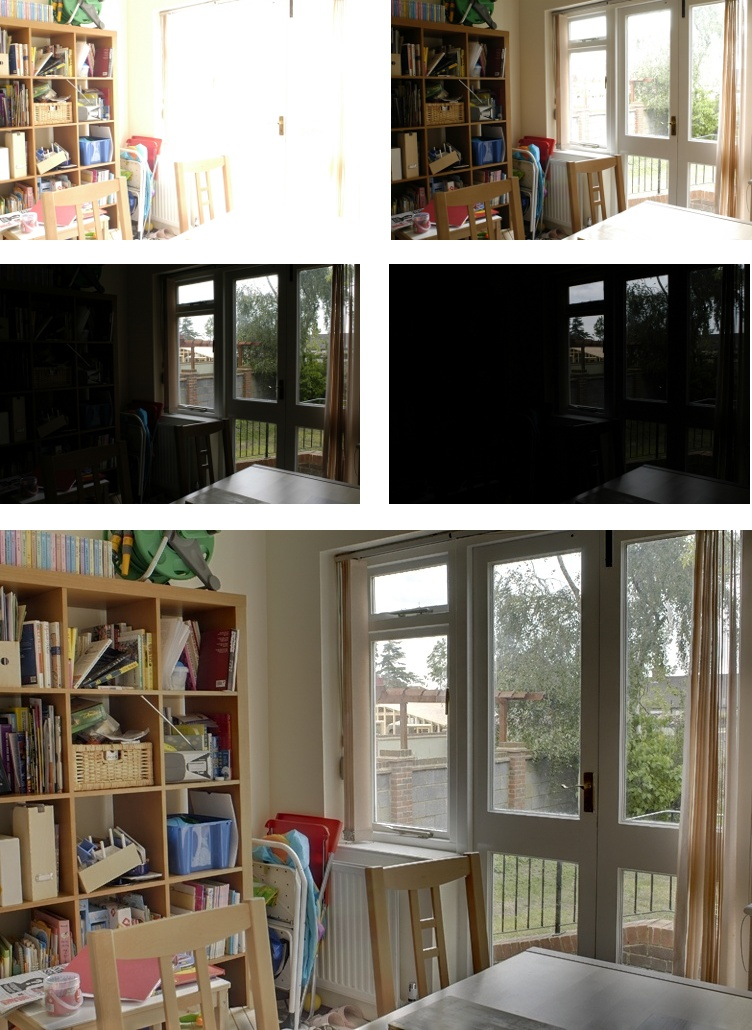
\includegraphics[width=\textwidth]{fused1.jpg}
        
        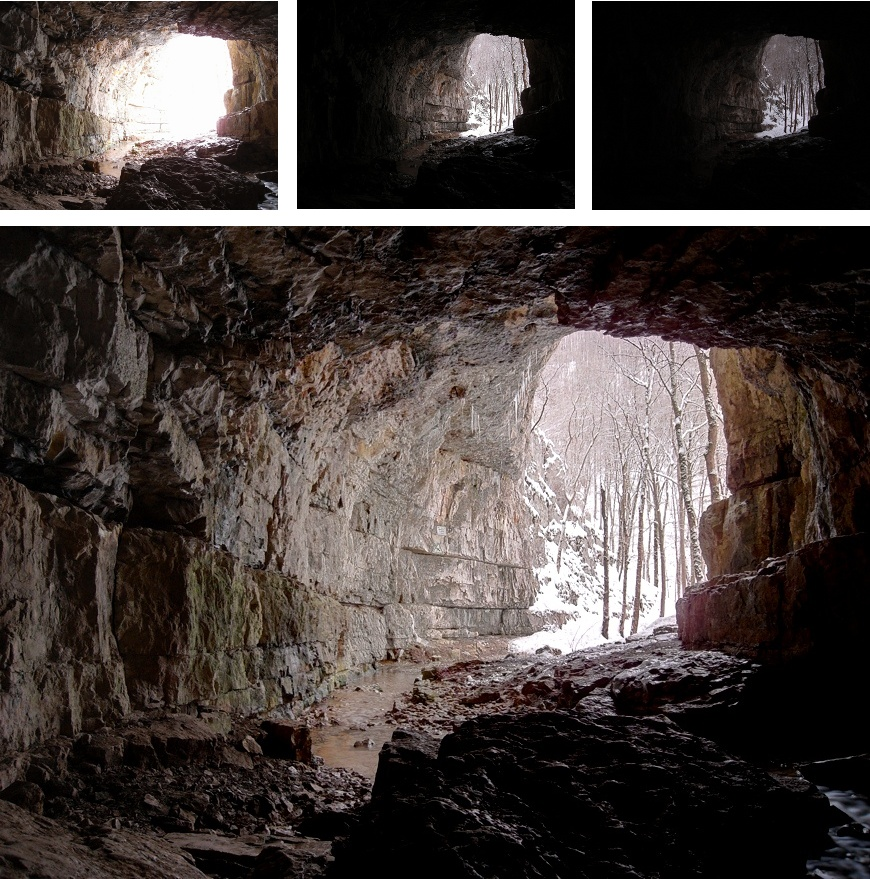
\includegraphics[width=\textwidth]{fused2.jpg}
        
        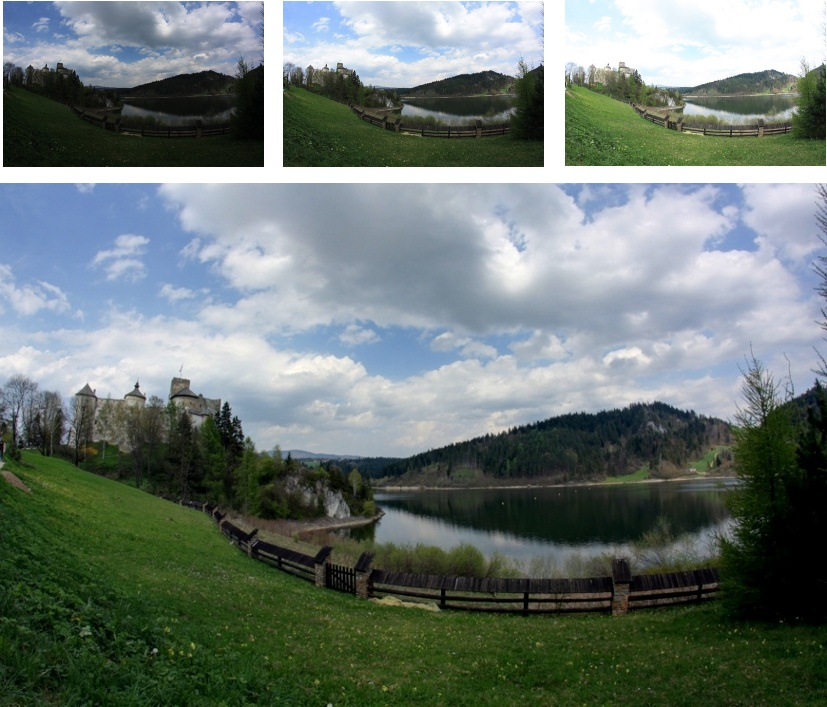
\includegraphics[width=\textwidth]{fused3.jpg}
        
        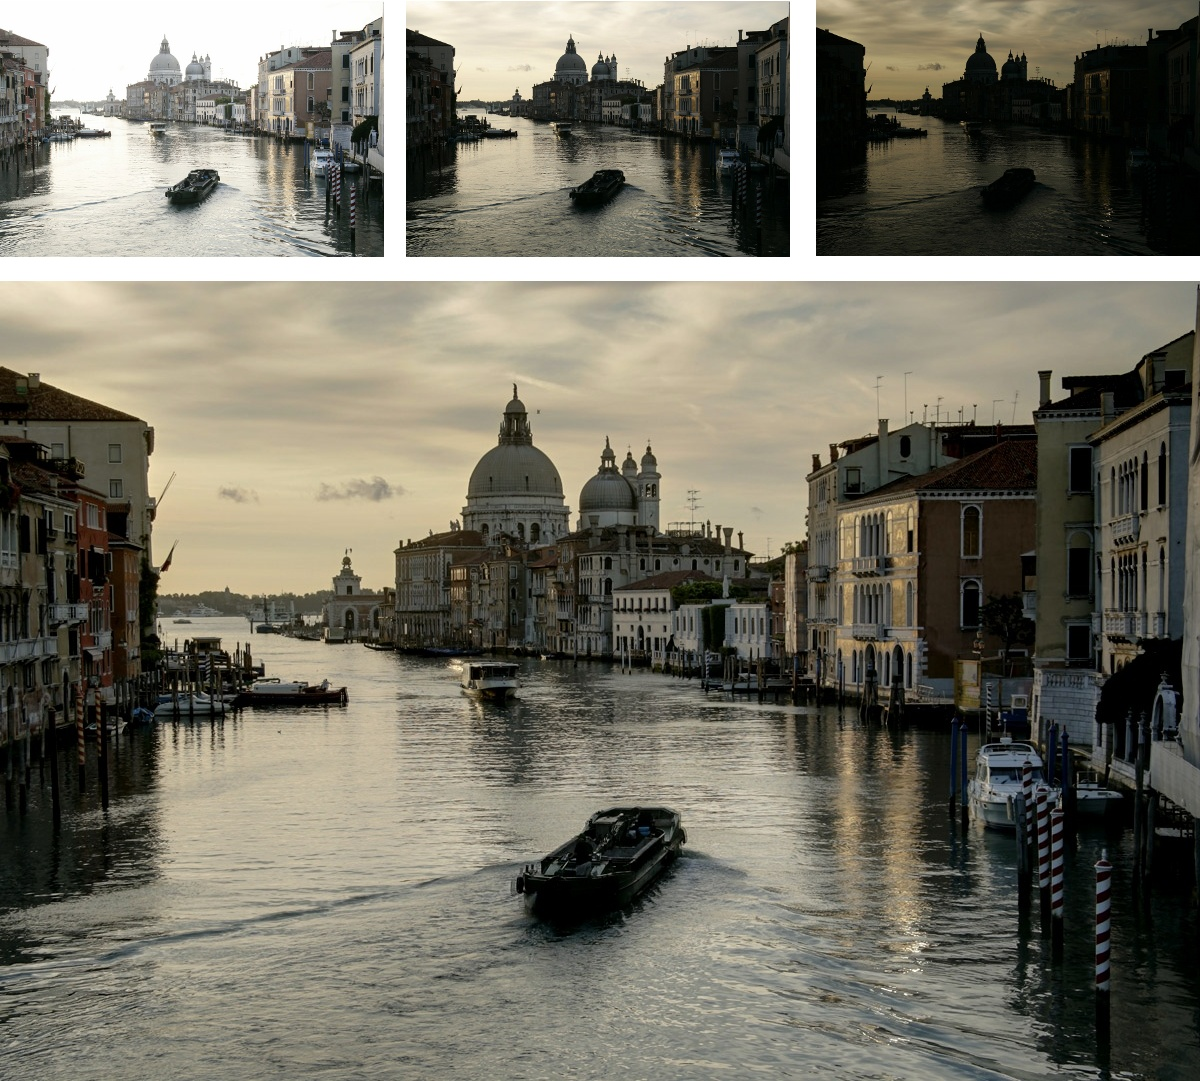
\includegraphics[width=\textwidth]{fused4.jpg}

    \section{Análisis de performance}
    
        A continuación mostrmos una tabla comparativa con los tiempos de ejecución del algoritmo implementado en Assembler y en C, para distinas imágenes de entrada. Se midió sólo el tiempo que tarda la ejecución del procesado, ignorando tiempos de cargado a memoria y guardado de imágenes.

        \bigskip
        \begin{tabular}{lll}
        \textbf{Cantidad y tamaño} & \textbf{C} & \textbf{ASM}\\
        4 $\times$ 752$\times$500 & 2.11s & 2.85s\\
        3 $\times$ 870$\times$653 & 2.46s & 3.27s\\
        3 $\times$ 1200$\times$800 & 4.15s & 5.54s\\
        5 $\times$ 1500$\times$750 & 7.68s & 10.34s\\
        3 $\times$ 3872$\times$2592 & 48.96s & 63.10s\\
        \end{tabular}
        \bigskip
        
        Se observa que en general la versión en Assembler tarda un 75\% del tiempo de la versión de C.

    \newpage
    \section{Compilar y Correr}
    
        La implementación tiene como dependencias la librería \textsc{OpenCV} y \textsc{Nasm}, que pueden instalarse en ubuntu con:\\
        \texttt{sudo apt-get install libcv-dev libhighgui-dev nasm}.
        
        Para compilar el proyecto, hay que correr \texttt{make} desde \texttt{/src}.\\
        \texttt{cd /src}\\
        \texttt{make}
        
        Si compila correctamente se puede correr el programa.
        \begin{itemize}
        \item Por consola, ejemplo:\\
          \texttt{./fuse -o room.jpg room/\{A,B,C,D\}.jpg}\\
          Corre el algoritmo con las imágenes \texttt{A.jpg}, \texttt{B.jpg}, \texttt{C.jpg}, \texttt{D.jpg} de \texttt{src/room/}.\\
          \texttt{./fuse -h}\\
          Para más información y detalle de los parámetros.
        \item Con la interfaz gráfica:\\
          \texttt{./gui}\\
          Inicia la interfaz gráfica donde se deben seleccionar las imágenes (seleccionar múltiples imágenes previamente alineadas y de las mismas dimensiones con \textsc{Ctrl}) y luego se pueden ajustar los parámetros y exportar la imagen final.
        \end{itemize}
        
        \subsection{Opcional: Alinear imágenes antes de fusionar}
            Para que el algoritmo funcione con los resultados esperados, las imágenes de entrada tienen que estar perfectamente alineadas.
            En general se obtienen las fotos con un trípode, variando la exposición de cada toma, pero sin mover la cámara.
            
            Pero también se pueden obtener las imágenes a mano alzada y luego alinearlas con un software. En este ejemplo mostramos cómo usar \texttt{align\_image\_stack} de \textsc{Hugin}.
            
            Primero, instalar las herramientas de \textsc{Hugin}:\\
            \texttt{sudo apt-get install hugin-tools}
            
            Luego, se pueden alinear las imágenes de la siguiente forma:\\
            \texttt{align\_image\_stack A.jpg B.jpg C.jpg D.jpg -a alineadas}\\
            Esto genera las imágenes alineadasXXXX.tif, que pueden ser usadas en la interfaz gráfica o por consola.

    \appendix

    \section{Rango dinámico}

        El rango dinámico en una cámara de fotos, se define como la razón entre el nivel de blanco más alto que puede detectar un sensor y el nivel más bajo. Los sensores de cámaras digitales en blanco y negro, consisten de una grilla de fotositos, que se pueden ver como un recipiente con capacidad para cierta cantidad de fotones. Luego de la exposición, se mide la cantidad de fotones que se encuentran en cada fotosito, y eso nos da el valor lumínico de cada pixel. Si nuestro recipiente se llena, decimos que el pixel esta saturado y va a detectar como valores iguales a todos los que esten por encima del máximo, luego, estamos perdiendo detalle en las zonas claras. Si disminuímos la exposición de la imagen para contrarrestar la saturación, estamos dividiendo la cantidad de fotones que inciden en un recipiente por algun factor, con lo cuál los valores que se encuentran en las zonas oscuras son cada vez más parecidos, y son mas indistinguibles del ruido electrónico generado al leer el valor, por lo que perdemos detalle en las zonas oscuras. Claramente el rango dinámico depende del tamaño de estos recipientes, por ejemplo las cámaras compactas, comparadas por ejemplo con SLR's profesionales, al ser mas chicas deben reducir el tamaño del sensor y por lo tanto el de los fotositos, disminuyendo así el rango dinámico. El rango dinámicos se mide con distintas unidades, de las cuáles la mas común es el f-stop, que describe el rango en potencias de 2, por ejemplo el rango $1024:1 = 1024 = 2^{10} f-stops$.
        En imágenes a color, simplemente tenemos 4 fotositos por pixel, donde cada uno detecta análogamente solamente en un rango de frecuencias cerca de rojo, verde o azul. 

    \bibliographystyle{plain}
    \bibliography{all}

\end{document}
